% Created 2021-01-18 lun. 09:10
% Intended LaTeX compiler: pdflatex
\documentclass[presentation]{beamer}
\usepackage[utf8]{inputenc}
\usepackage[T1]{fontenc}
\usepackage{graphicx}
\usepackage{grffile}
\usepackage{longtable}
\usepackage{wrapfig}
\usepackage{rotating}
\usepackage[normalem]{ulem}
\usepackage{amsmath}
\usepackage{textcomp}
\usepackage{amssymb}
\usepackage{capt-of}
\usepackage{hyperref}
\usepackage{color}
\usetheme{CambridgeUS}
\setbeamertemplate{navigation symbols}{} % pas de barre de navigation
\usepackage[english]{babel}
\usepackage{lmodern}
\usepackage[matha,mathb]{mathabx}
\usepackage{subfig}
\usepackage{mdframed}
\usepackage{minted}
\usemintedstyle{friendly} % set style if needed, see https://frama.link/jfRr8Lpj
\mdfdefinestyle{mystyle}{linecolor=gray!30,backgroundcolor=gray!30}
\BeforeBeginEnvironment{minted}{%
\small \begin{mdframed}[style=mystyle]}
\AfterEndEnvironment{minted}{%
\end{mdframed} \medskip \normalsize}
\usepackage{float}
\usepackage{url}
%% Formatting of verbatim outputs (i.e., outputs of R results):
\DefineVerbatimEnvironment{verbatim}{Verbatim}{%
fontsize = \small,
frame = leftline,
formatcom = {\color{gray!97}}
}
\setbeamertemplate{caption}[numbered]
%% Perso colors
\definecolor{PalePurple}{RGB}{127, 90, 182}
\definecolor{DarkPurple}{RGB}{98, 36, 134}
\definecolor{grey}{RGB}{51, 63, 72}
\setbeamercolor{title}{fg=white, bg=DarkPurple}
\setbeamercolor{frametitle}{fg=black}
\setbeamercolor{structure}{fg=PalePurple}
\setbeamercolor{section in head/foot}{fg=white, bg=PalePurple}
\setbeamercolor{subsection in head/foot}{fg=DarkPurple}
\setbeamercolor{title in head/foot}{fg=white, bg=DarkPurple}
\setbeamercolor{date in head/foot}{fg=grey}
\setbeamercolor{block title}{fg=white, bg=DarkPurple}
\setbeamercolor{block body}{bg=gray!20}
%% Structure of a slide :
\setbeamertemplate{footline}
{
\leavevmode%
\hbox{%
\begin{beamercolorbox}[wd=.75\paperwidth,ht=2.25ex,dp=1ex,center]{title in head/foot}%
\usebeamerfont{author in head/foot}\inserttitle
\end{beamercolorbox}%
%\begin{beamercolorbox}[wd=.3\paperwidth,ht=2.25ex,dp=1ex,center]{section in head/foot}%
%\usebeamerfont{title in head/foot}\insertsection
%\end{beamercolorbox}%
\begin{beamercolorbox}[wd=.25\paperwidth,ht=2.25ex,dp=1ex,center]{date in head/foot}%
\insertframenumber{} / \inserttotalframenumber\hspace*{1ex}
\end{beamercolorbox}}%
\vskip0pt%
}
\DeclareUnicodeCharacter{2514}{\mbox{\kern.23em \vrule height2.2exdepth-1.8ptwidth.4pt\vrule height2.2ptdepth-1.8ptwidth.23em}}
\DeclareUnicodeCharacter{2500}{\mbox{\vrule height2.2ptdepth-1.8ptwidth.5em}}
\setlength{\parskip}{6pt}
\usetheme{default}
\author{Frédéric Santos\thanks{frederic.santos@u-bordeaux.fr}}
\date{\today}
\title{Customizing and extending Emacs Speaks Statistics}
\hypersetup{
 pdfauthor={Frédéric Santos},
 pdftitle={Customizing and extending Emacs Speaks Statistics},
 pdfkeywords={},
 pdfsubject={},
 pdfcreator={Emacs 27.1 (Org mode 9.4.4)}, 
 pdflang={English}}
\begin{document}

\maketitle


\section{Introductory words}
\label{sec:orgd353a7d}
\begin{frame}[label={sec:org8c319d7},fragile]{A short tutorial for customizing ESS}
 \begin{block}{Target audience}
This tutorial is for R-users beginning to use ESS. We only assume that you have mild familiarity with Emacs, and that you know how to customize Emacs by filling your \texttt{.emacs} or \texttt{init.el} file.
\end{block}

\begin{block}{Goals}
\begin{itemize}
\item Helping newcomers and beginners to have a more friendly and efficient setup
\item Helping users migrating from other IDEs to keep behaviours and habits they are used to
\item Showcasing some other Emacs packages that play well with ESS and may improve your coding experience
\end{itemize}
\end{block}

These slides are a companion for the video tutorial available at \ldots{}
\end{frame}

\begin{frame}[label={sec:orgfd2d1e6},fragile]{An opinionated tutorial?}
 Some parts of this tutorial (e.g., replacing \texttt{Flymake} by \texttt{Flycheck} for syntax checking, or using \texttt{company} instead of other solutions for auto-completion) might be seen as quite opinionated. However, when several options or approaches were available for a given task, the most widespread and efficient (I hope!) was presented.

If you prefer other approaches, the ESS manual remains the canonical documentation: \url{http://ess.r-project.org/Manual/ess.html}
\end{frame}

\begin{frame}[label={sec:org15fecce},fragile]{A word about \texttt{use-package}}
 In this document, several pieces of Emacs Lisp code will be proposed so that you can use them in your init file.

It is assumed that you use \href{https://jwiegley.github.io/use-package/}{\texttt{use-package}} for your init file: the Emacs Lisp code can be adapted in a straightforward manner if you do not use it.

As a reminder, this is the minimal code to add in your init file so as to use \texttt{use-package}, once it has been installed:

\begin{minted}[]{common-lisp}
;; Make sure that use-package is installed:
(unless (package-installed-p 'use-package)
  (package-refresh-contents)
  (package-install 'use-package))
;; Load use-package:
(eval-when-compile
  (require 'use-package))
\end{minted}
\end{frame}

\section{ESS customization}
\label{sec:org8ee4a55}
\subsection{Visibility of evaluation}
\label{sec:orga87e6ce}
\subsection{Window management}
\label{sec:orgb839120}
\subsection{Syntax highlighting}
\label{sec:orgbf93b14}
\subsection{Parenthesis matching}
\label{sec:orge53ede3}
\begin{frame}[label={sec:org49491ca},fragile]{Seeing matching parentheses}
 Directly taken from the ESS manual (\url{http://ess.r-project.org/Manual/ess.html\#Parens}):

\begin{quote}
``Emacs has facilities for highlighting the parenthesis matching the parenthesis at point. This feature is very useful when trying to examine which parentheses match each other. This highlighting also indicates when parentheses are not matching.''
\end{quote}

To activate parenthesis matching in ESS[R] (source) buffers, add this to your init file:

\begin{minted}[]{common-lisp}
;; Activate global mode for parenthesis matching:
(show-paren-mode)
\end{minted}
\end{frame}

\begin{frame}[label={sec:orgdb6a798},fragile]{Navigating through matching parentheses}
 Here are some convenient tricks for navigating through parenthetical groups (this can be useful when dealing with large paren groups, e.g. when developing a shiny UI):

\small

\begin{table}[htbp]
\centering
\begin{tabular}{ll}
\hline
Shortcut & \texttt{Elisp function} (Docstring)\\
\hline
\texttt{C-M-p} & \texttt{backward-list} (Move backward across one balanced paren group)\\
\texttt{C-M-n} & \texttt{forward-list} (Move forward across one balanced paren group)\\
\texttt{C-M-SPC} & \texttt{mark-sexp} (Set mark at the end of the paren group)\\
\texttt{C-M-k} & \texttt{kill-sexp} (Kill from point to end of paren group)\\
\hline
\end{tabular}
\caption{Some useful shortcuts for dealing with parenthetical groups.}

\end{table}

\normalsize

For instance, when the point is over a closing parenthesis, \texttt{C-M-p} brings you to the matching opening parenthesis. Then, \texttt{C-M-k} kills to whole paren group.
\end{frame}

\subsection{Syntax checker}
\label{sec:org1d82ce8}
\begin{frame}[fragile,allowframebreaks,label=]{On-the-fly syntax checking}
 ESS has facilities for on-the-fly syntax checking. Instead of using \texttt{Flymake}, which is the default choice, using \texttt{Flycheck} appears to be a better and more stable option. To switch from Flymake to Flycheck, you can add the following in your init file:

\begin{minted}[]{common-lisp}
;; Remove Flymake support:
(setq ess-use-flymake nil)
;; Replace it (globally) by Flycheck:
(use-package flycheck
  :ensure t
  :init
  (global-flycheck-mode t))
\end{minted}
\end{frame}

\subsection{Rdired buffers}
\label{sec:org3fb0d37}

\section{Some useful Emacs packages}
\label{sec:orgfdcc02e}
\subsection{company}
\label{sec:orgc0fa105}
\begin{frame}[fragile,allowframebreaks,label=]{Completion}
 As mentioned \href{https://ess.r-project.org/Manual/ess.html\#Completion}{in the ESS manual}, there are several completion frameworks for writing R code with ESS. The Emacs package \href{https://company-mode.github.io/}{\texttt{company}} is an elegant solution, which also supports many other programming languages.

Here is a minimal piece of Elisp code to add in your init file to install and load \texttt{company}:

\begin{minted}[]{common-lisp}
(use-package company
  :ensure t
  :config
  ;; Turn on company-mode globally:
  (add-hook 'after-init-hook 'global-company-mode)
  ;; Only activate company in R scripts, not in R console:
  (setq ess-use-company 'script-only))
\end{minted}

\begin{figure}[htbp]
\centering
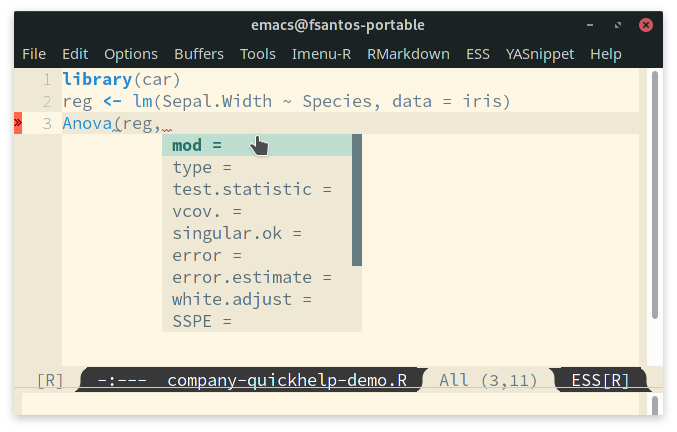
\includegraphics[width=0.72 \textwidth]{./images/company.png}
\caption{\label{fig:org4f865da}An example of code completion with \texttt{company}: various candidates are proposed for the arguments of the function \texttt{car::Anova()}.}
\end{figure}

\texttt{company} offers completion candidates in various contexts: function name, argument name within a function call (as in Fig. \ref{fig:org4f865da}), object name.

It may seem preferable to adopt a non-intrusive workflow. For functions or objects names, completion starts automatically after you type a few letters. For arguments names within a function call, it is suggested that you trigger manually the completion only when you need it. This can be done with \texttt{M-x company-complete}, or more conveniently, by binding this function to a convenient shortcut. For example, to bind it to \texttt{F12}, add the following to your init file:

\begin{minted}[]{common-lisp}
;; Use F12 to trigger manually completion on R function args:
(add-hook 'ess-r-mode-hook
	  '(lambda ()
	     (local-set-key (kbd "<f12>") #'company-R-args)))
\end{minted}

\pagebreak

Of course, further customization of \texttt{company} can be done in your init file. For instance:

\begin{minted}[]{common-lisp}
;; More customization options for company:
(setq company-selection-wrap-around t
      ;; Align annotations to the right tooltip border:
      company-tooltip-align-annotations t
      ;; Idle delay in seconds until completion starts automatically:
      company-idle-delay 0.45
      ;; Completion will start after typing two letters:
      company-minimum-prefix-length 2
      ;; Maximum number of candidates in the tooltip:
      company-tooltip-limit 10)
\end{minted}
\end{frame}

\subsection{company-quickhelp}
\label{sec:org06ffafe}
\begin{frame}[fragile,allowframebreaks,label=]{Documentation popups}
 \href{https://github.com/company-mode/company-quickhelp}{\texttt{company-quickhelp}} allows for documentation popups, e.g. to further describe function arguments.

\begin{figure}[htbp]
\centering
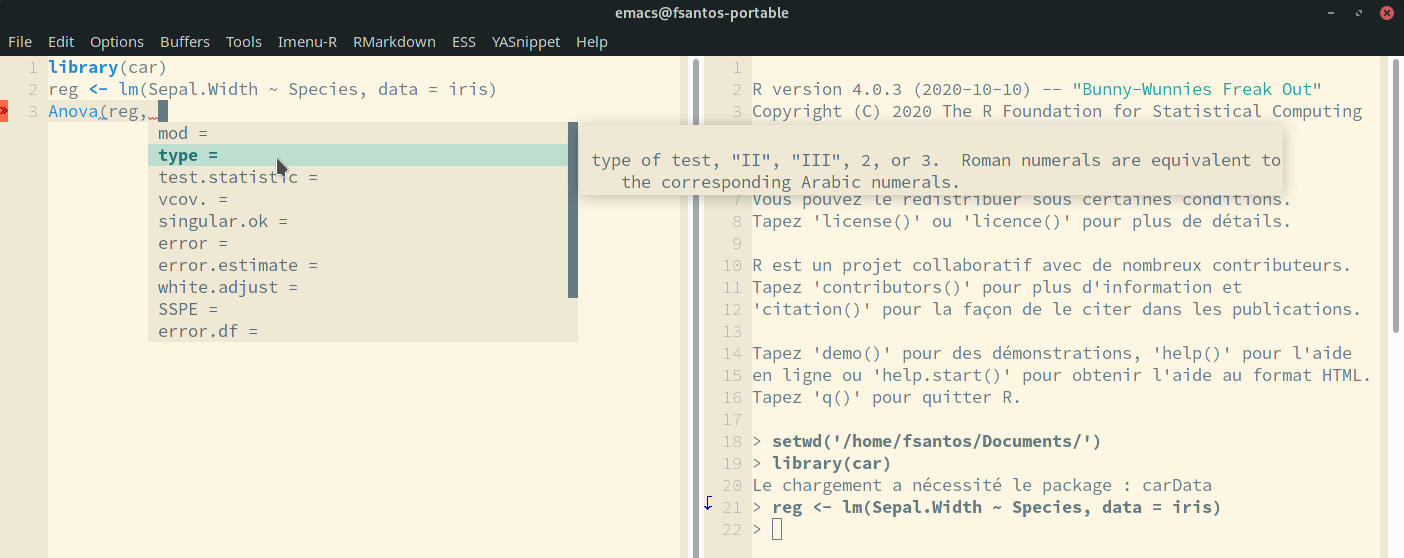
\includegraphics[width=\textwidth]{./images/company-quickhelp.png}
\caption{Documentation popups with \texttt{company-quickhelp}.}
\end{figure}

The minimal elisp code to add to your init file is straightforward:

\begin{minted}[]{common-lisp}
(use-package company-quickhelp
  :ensure t
  :config
  ;; Load company-quickhelp globally:
  (company-quickhelp-mode)
  ;; Time before display of documentation popup:
  (setq company-quickhelp-delay 0.3))
\end{minted}

By default, the documentation popup is shown automatically. You can adjust the time before the popup shows up by customizing the variable \texttt{company-quickhelp-delay}.
\end{frame}

\subsection{yasnippet}
\label{sec:orge0d9532}
\begin{frame}[label={sec:org2ee239c},fragile]{Code snippets}
 \href{https://github.com/joaotavora/yasnippet}{\texttt{yasnippet}} is an Emacs package allowing for the expansion of whole pieces of code you often use (\emph{snippets}) from one given abbreviation. 

\begin{block}{Key features of \texttt{yasnippet}}
\begin{itemize}
\item All code snippets are stored as plain-text files in one given directory, so that they are easy to share with other people, and can be easily version controlled.
\item As a corollary, it is also easy to retrieve and use large collection of snippets already available online. For instance, Andrea Crotti maintains a great collection available at \url{https://github.com/AndreaCrotti/yasnippet-snippets}.
\item Although we only demonstrate its use within ESS and R here, note that \texttt{yasnippet} is not an R-specific solution, and that you can use it for any other programming language.
\end{itemize}
\end{block}
\end{frame}

\begin{frame}[fragile,allowframebreaks,label=]{Setting up \texttt{yasnippet}}
 To set up \texttt{yasnippet}, proceed through the following steps:

\begin{enumerate}
\item Create a directory \texttt{snippets/} at some convenient location, and add a subfolder \texttt{ess-r-mode/} in this directory.
\item Add the minimal following code in your init file:
\begin{minted}[]{common-lisp}
(use-package yasnippet
  :ensure t
  :config
  ;; Indicate the directory containing your snippets:
  (setq yas-snippet-dirs '("path/to/your/snippets"))
  ;; Load your snippets on startup:
  (yas-reload-all)
  ;; Turn on yasnippet (minor) mode when editing R files:
  (add-hook 'ess-r-mode-hook #'yas-minor-mode))
\end{minted}
\item You can now fill your \texttt{snippets/ess-r-mode/} directory with your own snippets. For instance, create a file \texttt{function} (without any extension) in this directory, with the following contents:
\begin{verbatim}
#name : function
#key : fun
# --
${1:name} <- function(${2:args}) {
    ${3:body}
}
\end{verbatim}
Each snippet has a unique \texttt{name}, and can be triggered by typing a given \texttt{key} (followed by \texttt{TAB}). As we will see later on, the present snippet allows for the expansion of a template for defining new R functions more easily. The \texttt{yasnippet} manual gives more details about the expected syntax to define your own code snippets: \url{http://joaotavora.github.io/yasnippet/}.

\item Now your \texttt{snippets} directory should look like:
\begin{verbatim}
└── snippets
    └── ess-r-mode
        └── function
\end{verbatim}

Feel free to add or retrieve (a lot!) more snippets, i.e. to add more template files within the \texttt{ess-r-mode} sub-directory.
\end{enumerate}
\end{frame}

\begin{frame}[label={sec:orgcf0af66},fragile]{Using \texttt{yasnippet} in an ESS[R] buffer}
 While you are editing an R source file with ESS, each snippet can be triggered by typing its \texttt{key} and then pressing \texttt{TAB}. You can then navigate through the placeholders of the expanded template by pressing \texttt{TAB} again.

For instance, with our previously defined snippet, typing \texttt{fun} followed by \texttt{TAB} will expand the full \texttt{function} template; you will then be able to specify easily a value for each of the three placeholders (the function's \texttt{name}, its \texttt{args} and \texttt{body}).

Note that \texttt{yasnippet} has a short video tutorial, available at \url{https://www.youtube.com/watch?v=ZCGmZK4V7Sg}.
\end{frame}
\end{document}